% Changing book to article will make the footers match on each page,
% rather than alternate every other.
%
% Note that the article class does not have chapters.
\documentclass[10pt,twoside,twocolumn,openany]{book}
\usepackage[bg-letter]{dnd} % Options: bg-a4, bg-letter, bg-full, bg-print, bg-none.
\usepackage[english]{babel}
\usepackage[utf8]{inputenc}
\usepackage{graphicx}
\graphicspath{{img/}}

% Start document
\begin{document}
\fontfamily{ppl}\selectfont % Set text font

% Your content goes here

% Comment this out if you're using the article class.
\chapter{Wulf: A Retelling}

\section{Introduction}
\textit{Wulf} is a "historic fiction fiction" campaign loosely based on the beginning of the epic \textit{Beowulf}. This campaign is designed for four level 5 players using the 5th Edition D\&D ruleset. The campaign is set in and around northern Europe as far as mapping goes.

\section{Plagued by Demons}
Our story begins with the tragic tale of King Hrothgar of Denmark. As a ruler, Hrothgar has been both brutal to his enemies and just to his countrymen. Now made wise with age and laden with hard won treasures, Hrothgar has retired from the conquering life and settled down as a less hands on ruler in his great hall, Herot. This hall is built to a scale and decadence never before seen in this part of the world. Travelers and rulers from all around the region come to pay tribute, dine, and revel in Herot. However, this bliss was not destined to pass. 

Not long after Herot's completion talk of a monster marauding through the nearby hills spread through the hall. This entity, called Grendel by the Danes, appears closer to Herot each night and, after a fashion, storms the great hall. Grendel enters after sundown, slaughtering many of the people now cornered inside Herot. He then consumes the corpses of his victims, then leaves just before sunrise.

Many brave warriors have traveled to Herot to win glory by killing Grendel. As a result of this Grendel has remained relatively well fed. Each night Herot and the surrounding towns are left abandoned in an attempt to preserve some sense of safety, but Grendel grows ever more hungry and violent towards the Danes.

\section{Foreign Direct Investment}
Nearby, in G{\"o}taland, an enterprising ruler sees an opportunity for investment. Higlac, king of the Geats, knew that if he sent a group of his followers to slay the monster Grendel that Hrothgar would not only pay in treasures but be left with a debt of gratitude to the Geats.

Not more than a week ago, Higlac rounded up a group of his followers best suited to the task. He set them on a boat with a course for Denmark. This is where our story begins in earnest, a few miles off Danish shore.

\begin{commentbox}{Adventurer's Background}
The players can be of any race or class, or have any background in general. However, a few commonalities must be shared. Each character must at least reside in G{\"o}taland prior to the beginning of the campaign. Besides that, everything is negotiable. Some adventurers may be members of King Higlac's court, or soldiers, folk heroes, or especially skilled common folk.
\end{commentbox}

\clearpage

\chapter{1: In Herot's Walls}

\section{Seeking Shore}
This adventure begins as many, on a boat to a foreign land. The party has recently been conscripted to travel from G{\"o}taland to Denmark by order of King Higlac to kill the monster Grendel. The trip itself is over calm waters and end without any real incidence. The ship is now nearing Danish land, and the party has some time between daily ship's tasks, their first actually free moments since leaving dock.

Soon, in early morning, the ship is upon the shores. The party lays anchor and send out a dingy to land. Once ashore, a soldier on horseback will come down from a nearby watchtower to meet the party. The guard will ask the adventurers why they are entering Danish land, as no travelers were expected. Upon learning they were sent by Higlac, a ruler friendly towards the Danes, the adventurers will be allowed to pass into Denmark. Herot lies just inland from where the party beached.

\begin{commentbox}{NPC Backgrounds}
\textbf{Hrothgar}: Longtime king of Denmark. In his youth, Hrothgar was a powerful and skilled warrior. He has a good working relationship with Higlac, king of the Geats. While Hrothgar hasn't personally heard of the adventurers, he knows that Higlac would only send warriors of the highest possible caliber. As such, Hrothgar is optimistic about the adventurer's ability to kill Grendel.
\\
\textbf{Unferth}: Retainer to King Hrothgar, Unferth was in Herot when Grendel first attacked. He saw first hand the savageness of Grendel, and feels a very primordial fear of the monster. He also observed that no weapon can harm the beast. Unferth holds the belief that Grendel is an agent of the gods sent to punish the Danes for their decadence. Further, Unferth holds that the only way to rid themselves of Grendel is to abandon or destroy Herot. Despite his lobbying, Hrothgar refuses to listen to Unferth's concerns.
\\
\textbf{Aeschere}: Hrothgar's close friend and most trusted warrior and advisor. While he is both well traveled and educated in both martial and academic arts, recent events have made him distrustful of outsiders. He has watched as many warriors come to Herot to challenge Grendel, and all have failed. Most of the warriors have been glory seekers hoping to use the Dane's misfortune as a means to gain fame and riches.
\end{commentbox}

\section{Cite of Struggle}
The adventurers soon reach the town surrounding Herot. On the outskirts of the town the adventurers will pass by a large field filled with freshly made graves.

\begin{quotebox}
Near the road you see a man and a woman standing over one of the most recently dug graves. The woman, in funeral garb, is weeping. Her companion, Unferth, is consoling her as best he can.

"There was nothing anyone could have done. Grendel is not a beast that can be reasoned with or slain. At least Agner won't have to see any more of the horror that has befallen us. I told Hrorthgar we need to abandon Herot, maybe soon he will finally listen."
\end{quotebox}

The mourners are Unferth, one of Hrothgar's retainers, and Agathe, his sister. The grave belongs to Agner, Agathe's young son who was ripped to shreds by Grendel in his sleep the previous night. Unferth believes that Grendel is a form of divine retribution sent by the gods to punish Hrothgar for the decadence of Herot. As such, Unferth believes that nothing short of destroying or abandoning Herot will rid them of Grendel. He laughs at the mere mention of any other resolution.

As the adventurers trek further into the town they will see other signs of conflict; burned and partly broken buildings dot the streets, and few people are seen outside of their homes. Herot lies atop a knoll in the center of the town. Servants are cleaning blood from the steps of the great hall as the party approaches.

Herot itself is a towering structure, standing at least three stories high. Its walls and roof appear made out of finely worked wood with intricately carved detail work dotting the structure.

\section{The Greatest of Halls}
As the party enters Herot their way will be stopped by Aeschere, Hrothgar's most loyal and trusted soldiers. Aeschere is a powerful warrior and insightful advisor, but recent events have made him cast a wary eye at outsiders.

\begin{quotebox}
Aeschere, a fearsome looking warrior, blocks your way as you enter Herot.

"Who dares enter my Lord Hrothgar's great hall in this time of tragedy!"

Behind Aeschere and atop a throne, Hrothgar motions for you to enter.

"Let them be, Aeschere. There is nothing worse they could do than has already been done."
\end{quotebox}

The interior of Herot is, or was, lavish to the point of near absurdity. While it appears that most surfaces were recently cleaned there are still signs of destruction. The banners that are still holding to the walls are torn, the hall's floor and walls are gouged in places, and some detritus can still be seen in distant corners of the hall. Herot is comprised of a single large room, its ceiling reaching a full three stories high at the center of the room. At the extreme end of the hall, opposite the doors, sits the king's tall throne. Between the throne and the door stretches an appropriately massive banquet table with bench seating on either side.

Hrothgar will invite the adventurers to approach his throne and ask if they have come to his aid. Hrothgar will light up upon hearing that they were sent by Higlac. The Danes keep a good working relationship with the Geats, and Hrothgar trusts that Higlac would only send truly powerful warriors to his aid. Elated, Hrothgar announces that a feast will be held this afternoon to honor the adventurers and prepare them for their upcoming trial.

\section{Revel and Revelation}
Shortly after noon the feast starts. Hrothgar sits at the head of the table with Aeschere at his side, while Unferth sets out food for the gathered crowed. In addition to the adventurers, seated near Hrothgar's end of the table, a group of 15 or 20 Danish soldiers has joined in the feast. It is easy to tell, however, that the hall was made to hold many times more people, and more would have attended any feast in Herot if it wasn't for fear of Grendel.

The spread consists of bread, stews, and roast and cured meats and fish. Unbeknown to all in attendance, Unferth has tainted some of the stew with a torpor poison. Obviously, Unferth will try to avoid poisoning himself. Once the guests have eaten and start to take ill from the poison a disgruntled Unferth will claim this illness as another sign from the gods and try to convince the king to destroy or abandon Herot.

\begin{quotebox}
Unferth, as if on cue, forcefully stands up from his seat at the table just as the other revelers start to take ill. "Behold, most noble King! Can you not see the signs now? Grendel has already been sent by the gods as divine punishment for the decadence of this hall. Many of your own people have already perished or ran. This sickness must be another facet of the gods' divine punishment! Will you not listen to my pleads now? We must either destroy Herot or abandon the city. Only then will your people be safe once more!".
\end{quotebox}

\begin{paperbox}{}
\textbf{Torpor (Ingested)}. A creature subjected to this poison must succeed on a DC 15 Constitution saving throw or become poisoned for 4d6 hours. The poisoned creature is incapacitated. An incapacitated creature can't take actions or reactions.
\end{paperbox}

Both Hrothgar and Aeschere are at a loss. Neither of them had initially believed Unferth's claims that Grendel has been a form of punishment from the gods, but the sudden illness at this revel is adding credibility to Unferth's argument. However, this is not enough evidence to push the king onto another course of action.

\clearpage

\section{\textbf{Grendel}}
A monstrosity that slumbers in a subterranean lair by day, and hunts by night, Grendel exists as a true example of decadence and evil. Each night Grendel must feed on a fresh kill in order to sate his unending hunger for flesh. Many believe that Grendel is, in fact, the distant descendant of a human. However, somewhere along the lineage a corrupting influence fundamentally changed one of his ancestors.

Unable to be harmed by weapons, Grendel can only be killed in hand-to-hand combat. However, he can more than defend himself from any eventual unarmed conflict. His ravenous claws can easily slay most creatures. And once he is injured he can use the flesh of his combatants to heal himself.

\vspace{4.1cm}

\begin{monsterbox}{Grendel}
	\textit{Huge monstrosity, chaotic evil}\\
	\hline
	\basics[%
	armorclass = 12,
	hitpoints  = 105 (10d12 + 40),
	speed      = 60 ft
	]
	\hline
	\stats[
    STR = \stat{25},
    DEX = \stat{8},
    CON = \stat{19},
    INT = \stat{5},
    WIS = \stat{10},
    CHA = \stat{7}
	]
	\hline
	\details[%
	% If you want to use commas in these sections, enclose the
	% description in braces.
	% I'm so sorry.
	senses = {darkvision 60ft., passive Perception 16},
	languages = {Common, Abyssal},
	damageimmunities = {Any armed attacks},
	damageresistances = {Magic},
	challenge = 5
	]
	\hline \\[1mm]
	\begin{monsteraction}[Multiattack]
		Grendel makes two Claw attacks.
	\end{monsteraction}\\
	\begin{monsteraction}[It Bleeds]
		While bloodied, Grendel looses 1d6 hit points each round.
	\end{monsteraction}
	\monstersection{Actions}
	\begin{monsteraction}[Claw]
		\textit{Melee Weapon Attack}: +8 to hit, reach 10 ft., one target. \textit{Hit}: 18 (3d8 + 5) slashing damage.
	\end{monsteraction}

	\begin{monsteraction}[Consume]
    	Grendel grapples with a target within 10 ft. On a success, Grendel can consume a chunk of the victim. The target takes 18 (3d8 + 5) piercing damage, and Grendel regains the same amount of hit points.
	\end{monsteraction}
\end{monsterbox}

\begin{figure}

	\vspace{-4.5cm}
	
	\centerline{
		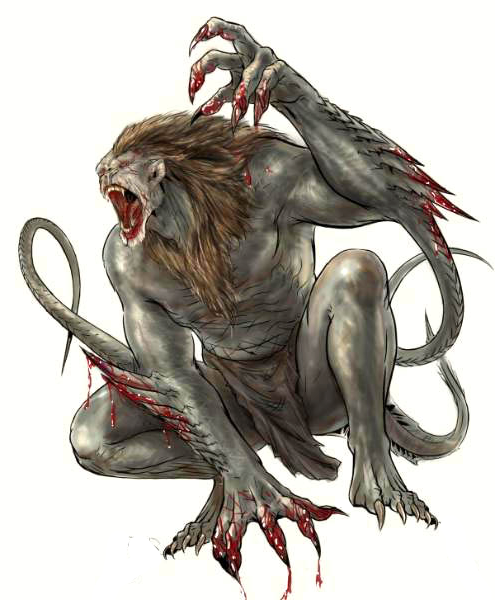
\includegraphics[scale=1]{grendel}
	}
\end{figure}


\clearpage

\end{document}
